\documentclass[a4paper]{thesis}
\usepackage[a4paper,top=2cm,bottom=2.5cm,left=1.5cm,right=1.5cm,marginparwidth=1.75cm]{geometry}
\usepackage[english]{babel}
\usepackage[utf8x]{inputenc}
\usepackage{amsmath}
\usepackage{graphicx}
\usepackage{wrapfig}
\usepackage{microtype}
\usepackage{setspace}
\usepackage{enumitem}
%\usepackage{fixltx2e}

\usepackage[nottoc]{tocbibind}
\usepackage{natbib}
\usepackage[section]{placeins}

\title{\Large{\textbf{Virtual 3D Scanner}}}
\author{Esteban Andrade\\ 
12824583}
\date{\today}

\setstretch{1.25}
\graphicspath{ {./images/} }
\bibliographystyle{agsm} %agsm

\begin{document}





\section*{\centering{Background}}
As human society in general, the comprehension of the surrounding world is mainly determined with visual perception.
This will allow us to distinguish different kind of shapes, objects, textures, colours, and the spatial locations of our surroundings.
With this information we can analyse the number of objects in a specific location, the type of the objects, the corresponding sizes, their distances with respect to different coordinates frames.
Which impact how we can interact with an object or scene.Therefore, the imitation of these senses in engineering designs and implementations, will allow to gather real world data for many kinds of applications, involving the use of several kind of sensors and data format types that include: 
 \begin{itemize}
    \itemsep0em 
     \item Traditionally images
     \item Depth images
     \item Multispectral images
     \item 3D point clouds 
 \end{itemize}
 Based on the data obtained with these types of sensors, there are several possible ways to use computer processing techniques.Depending on the task, to model accurate objects or subjects for different applications as suggested by Murcia, Monroy and Mora,( 2018). 
 Nowadays one of the approaches that has been developed based on this concept is to develop 3D model of human bodies using different techniques and sensors.
 This methodology is commonly known as “Body Scanning” and is becoming widely used in a variety of industries, especially on the fashion industry. 
 
 \section*{\centering{Industry Approach}}
 As mentioned before the advancements of 3D body scanning has gained importance. One particular example is within the clothing industry, as it has raised the demand for high quality, short production times and low manufacturing cost. 
 With the use of 3D Scanners, it will help manufactures from around the world to acquire correct data measurements of body dimensions. 
 As stated by Sturm, Bylow, Kahl and Cremers, (2013), this new technology approach could change drastically the future of how the entire clothing and fashion industry operates.\\[10pt]
 One of the crucial issues for the clothing industry is to create better fittings for human bodies.
 With the innovation of 3D image modelling technology, there has been a noticeable interest from this industry to obtain accurate measurements of the human body.
 Similarly, with the gathered data from these scans, there has been the raise of Virtual try on solutions for both Online and Retail stores (Spahiu, Shehi and Piperi, 2014). 
 Hence, allowing to extract tailoring measurements straight from the Scans, which would allow to massively reduce the custom tailoring process. \\[10pt]
 This is particularly used in garment design and body shape analysis. Allowing manufactures to improve the sizing and fitting of their range of products. 
 Thus, it will reduce the amount of imperfections and potential sizing issues with customers. 
 As a result, it will increase the overall benefits of the fashion and sizing industry and increase customers satisfaction among the buyers of their products by taking accurate measurements of their body with a scan. 
 Therefore, allowing them to know how the specific piece of clothing will look like with the recreated model of their body. 
 \enlargethispage{\baselineskip}


 \subsection*{Other Approaches}
 3D Scanners have also grown in participation in other industries. The  characteristic that these systems are low cost and non-invasive are making this technology  appealing for a widespread clinical uses and epidemiological surveys (Treleaven and Wells, 2007).\\[10pt]
 In the clinical aspect the scanning application can be divided into geometry measurements and texture visualization. 
 Geometry measurements is associated with size, shape, surface area and volume. Whereas texture visualization comprehends regions of the body like head, chest, rest of the body.
 Based on gathered data from this criterion different healthcare applications can be formed and include: 
\begin{itemize}[]
    \itemsep0em 
    \item Epidemiology
    \item Diagnosis
    \item Treatment
    \item Monitoring
\end{itemize}
The table below demonstrated the use of 3D scanner in the medical field with the objective to detect and monitor various medical conditions. In which it suggests how to diagnose, treat, and monitor different results based on the acquired data.
\begin{table}[ht]
    \centering
    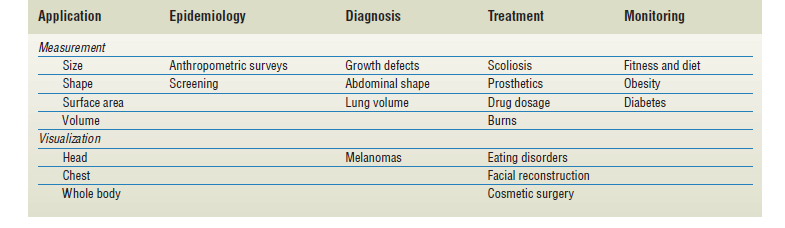
\includegraphics[width=17cm]{table1.png}
    \caption{3D Scanning Applications \cite[]{treleaven_wells_2007}.}
\end{table}

\begin{figure}[h]
    \begin{center}
    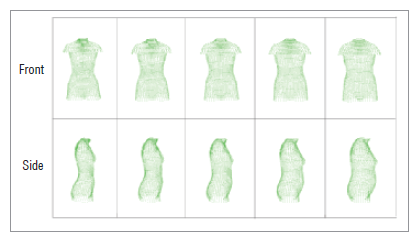
\includegraphics[width=0.5\textwidth]{bodyMedicine.png}
    \caption{Front, Side results of 3D Scanning \cite[]{treleaven_wells_2007}.}
    \label{bodymed}
\end{center}
\end{figure}
Additionally, 3D Scanning could be suitable to screen children with obesity, growth defects or deformities.
Therefore, the use of 3D scanning for medical application can help health authorities to track different anomalies that patients may have.
It will ease the process to diagnose, treat and monitor different kind of medical conditions and improve the quality of life of the patients with non-invasive tests. \\[12pt] 
\enlargethispage{\baselineskip}


\section*{\centering{Economic Impact}}
One of the critical aspects of the clothing industry, especially on E-Commence, is the return rate due to sizing issues. Normally the return rate is between 60\%-70\%.
Therefore, the massive loss of revenue to companies of this sector a problem worth solving. 
The average percentage of a total sale due to shipping is around 5\% of the total sale. 
If for instance the item must be returned due to a problem of sizing and fittings then the total shipping cost will increase drastically, as mentioned by Gonzalez-Rodriguez, (2020). 
Hence, reducing the total profit per item and decreasing the total net Revenue.\\[10pt]
It is estimated alone, that only in the United States the sizing issues causes a net total cost of 550 billion USD on return cost, this does not include restoking expenses nor inventory losses.
The size and fit took a significant percentage of this total estimate, as it was noticed that around 50\% of customers will purchase different sizes, with the intention to return some of them.\\[10pt]
Thus, it is imperative that with the use of 3D body scanners, the total losses due to sizing issues will be decreased drastically and it will reduce the total amount of economic losses.
On the other side, with the use of these systems it will make the purchase process much more “pain free” and enjoyable for the customers. Since it will allow them to try virtually and in real time the piece of clothing that they are willing to purchase.

\section*{\centering{Engineering Design Brief}}
Been able to scan different subjects and objects has been challenging, for researchers, especially to get accurate spatial locations of points in objects. The use of 3D point clouds has gained popularity in this field, as the data provides information of a scan with the following parameters: 
\begin{itemize}[]
    \itemsep0em 
    \item Depth
    \item Intensity
    \item Pulse width
    \item Light echo
\end{itemize}
All this information will depend on the kind of sensors used for the scanning. Currently, there is a wide variety of off-the shelf sensors that provide 3D point clouds data based on stereo or Multiview vision Cameras , lasers scanners, time-of-flight sensors cameras and structured light sensors (Murcia, Monroy and Mora, 2018). 
Additionally, the use of Lidars, either 2D or 3D, have grown significantly with the grown popularity of this new technology.
Many Scanning systems will be based on either one or multiple of the above-mentioned sensors. 

\subsection*{Technological Context}
One of the methods and techniques that has been developed for 3D scanning and tracking is names as “Dynamic Fusion”. Which is based on reconstruction and tracking of Non-rigid Scenes in real time (Newcombe, Fox and Seitz, 2015).
This is a revolutionary method based on SLAM (Simultaneous Localization and Mapping), which is adapted to Dynamic Scenes.\\[10pt]
%\begin{wrapfigure}{r}{0.55\textwidth} %this figure will be at the right
%    \centering
%    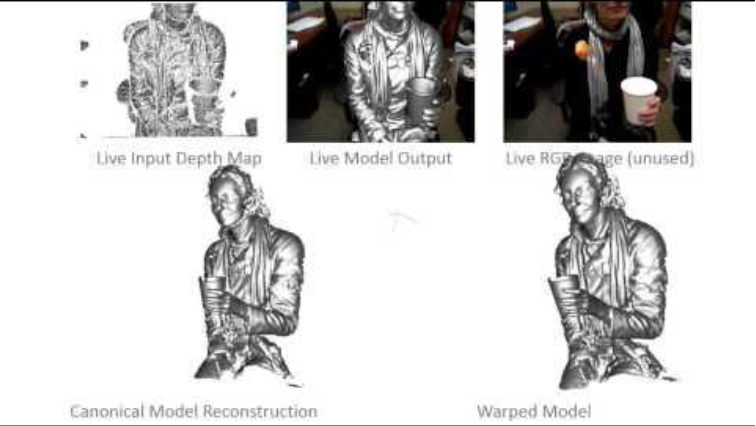
\includegraphics[width=0.5\textwidth]{dynamicfusion1.png}
%    \caption{pretty picture}
%\end{wrapfigure}
The basic principle of the reconstruction of non-rigid Scenes is obtained by fusion data from an RGB-D sensor camera.
This type of sensors provides images in 3 channels RGB (red, green, blue), and the depth maps are given by each pixel. 
All this data could be analysed and converted to the subsequent 3D point clouds for processing.
Dynamic fusion is the mesh and fusion of three techniques used for 3D scanning and reconstruction.  These techniques are:

\newpage
\begin{description}[style=nextline]
    \item[Kinect Fusion] Used for real-time Dense surface Mapping and tracking. This technique is designed for static scenes and objects only with a moving camera
    \item[DART (Dense Articulated Real Time Tracking)] This technology is focused on Real Time template tracking.
    \item[Animation Cartography] 3D reconstruction technique used for intrinsic Reconstruction of shapes and motions. 
\end{description}

\begin{wrapfigure}{r}{0.5\textwidth} %this figure will be at the right
    \centering
    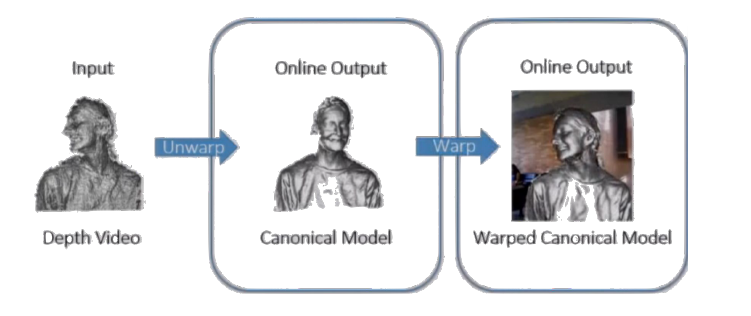
\includegraphics[width=0.5\textwidth]{IMG_0073.png}
    \caption{Transformation Between Depth Video to Warped canonical Model. \cite[]{newcombe_fox_seitz_2015}}
\end{wrapfigure}
The principal focus of Dynamic fusion, 3D reconstruction technique, is that once the data is gathered, it will solve for a volumetric flow field. 
This will transform the state of the scene at each time instant into a fixed canonical frame as developed by Newcombe, Fox and Seitz (2015). \\[10pt]
The canonical frame is known as the first frame that is captured from the non-rigid object that has been tracked and scanned. The canonical model is the shape of the object that is defined in the canonical frame. 
Thus, the canonical model will be used as reference for other frames and there will be cumulative refinement on this model and frames, as more scans and  measurements are taken.
With the new refinements each point in the canonical frame, which will be point cloud will be transformed to its new location in the real time frame.\\[10pt]
The volumetric flow field will be estimated with the help of the warp field parameters using the live depth video from the sensors. 
The state of the wrap field W\textsubscript{t} is defined as a function of time and defined by the values of a set of n deformation nodes, which are points in the actual image
\[N_{warp}^t=\{dg_v,dg_w,dg_{se3}\}t\]
\begin{itemize}[label =]
    \item $dg_{v}$: Used for real-time Dense surface Mapping and tracking. This technique is designed for static scenes and objects only with a moving camera
    \item $dg_{se3}$: This technology is focused on Real Time template tracking.
    \item $dg_{w}$: 3D reconstruction technique used for intrinsic Reconstruction of shapes and motions. 
\end{itemize}
The current level set of point clouds will be stored as a polygon mesh, with normal pairs points in the canonical frame, that later will be used for surface reconstruction.   
Slavcheva, Baust and Ilic, (2018)  mention that once the warp field parameters are obtained from the data, the surface reconstruction can be modelled using Marching Cubes, followed by the rasterization rendering pipeline of the Acquired Point cloud values.\\
\begin{wrapfigure}{r}{0.25\textwidth} %this figure will be at the right
    \centering
    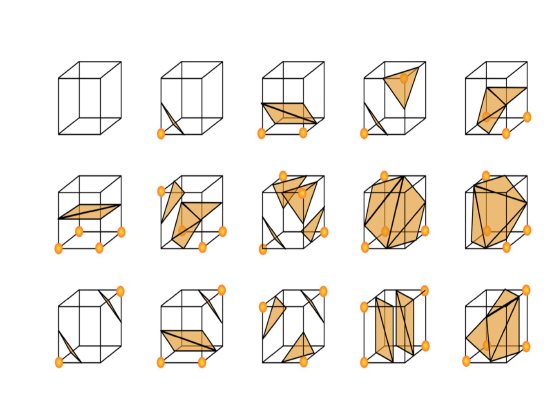
\includegraphics[width=0.21\textwidth]{shapes.png}
    \caption{Triangulated patterns \cite[]{fang_zhao_wen_zhang_2018}}
\end{wrapfigure}
These 15 patterns from the image 3 represent the Triangulated cubes for the 15 basic patterns used in Marching Cubes for the method of surface reconstruction. These patterns can reconstruct all the 256 possible solutions using complementary and rotational symmetry (Fang, Zhao, Wen and Zhang, 2018).
\begin{figure}{l} %this figure will be at the right
    \centering
    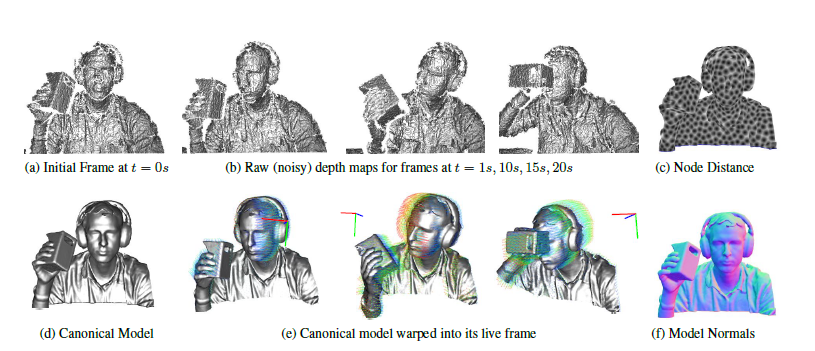
\includegraphics[width=0.7\textwidth]{dynamicfusion2.png}
    \caption{Dynamic Fusion methodology \cite[]{newcombe_fox_seitz_2015}}
\end{figure}
Once the canonical model, and frame and warp field parameters are obtained from the initial data frame and raw depth maps, the nodes will be created. Then the canonical frame warp parameters will be estimated. Once the canonical model is created it will be warped to its live frame with help of the warp parameters and then the model normalised and is created. \\
\enlargethispage{\baselineskip}

\section*{{Limitations}}
There are a few uncertainties 3D scanning technologies. One example is that most 3D scanning technologies can not be performed in real life and it will require the subject to be static. Therefore, causing uncertainties on how the model will be affected in different positions and orientations as stated by Fang, Zhao, Wen and Zhang (2018).\\
Regarding dynamic fusion, one of the limitations is that reconstructions of highly dynamic scenes leads to instability of the warp field and its corresponding parameters. Thus, causing issues in modelling the canonical model.  (Newcombe, Fox and Seitz, 2015)\\
Additionally, as the size and complexity of the scenes and objects increases, the problem of predicting the occluded areas becomes more difficult to model properly. \\
Furthermore, the memory size of the data will increase as the precision and accuracy increases, hence demanding more computational resources. 
\subsection*{Uncertainties and Risks}
With the current development of different techniques and technologies used for 3D scanning there are a few uncertainties and implications of this project. \\[10pt]
In an ethical perspective, it is noticeable that there is no clear guidance or legal framework that will regulate the use of the gathered data. Therefore, there is the potential of Data losses of different users of this technology that can be used in many ways. \\[10pt]
On the other side, there are a few risks and uncertainties in the technical side. These include what kind of hardware to use as this will range from RGB-D Cameras, lasers, Time-of-flight sensors, and many other ways to gather data. Also, what kind of software and tools will be used to control and fuse the data.
 Possible implementations include ROS, OpenCV, CUDA, etc. Thus, there is no certainty on how to approach this problem and it will be subjective to each researcher or developer on how to implement a solution depending on the specific scenario. \\ [10pt]
Additionally, there is the latent risk that this technology would not become available to the market in general. Therefore, putting all the development at risk. On the other side, there is the risk that people in general would not take part of this technology. As it is not know what the adoption rate will be for customers in general to be scanned and use that data for different applications, that could range from the fashion industry to health. 

\newpage


\nocite{*}   % all not cited bib entrys are shown in bibliography ...
\bibliography{resources}

\end{document}